
\chapter{Introduction to Minsky}

\label{Introduction-Minsky}

\emph{Minsky} is a system-dynamics program. If you are familiar with
these programs, please go to \ref{intro:experienced-system-dynamics}.
If you are not, please go to \ref{intro:new-system-dynamics}

\section{If you are new to system dynamics}

\label{intro:new-system-dynamics}

\emph{Minsky} is one of many ``system dynamics'' programs \url{https://en.wikipedia.org/wiki/System_dynamics}.
These programs allow a dynamic model of a system to be constructed,
not by writing mathematical equations or computer code, but by laying
out a model in a block diagram, which can then be simulated. These
programs are now one of the main tools used by engineers to design
complex products, and by management consultants to advise on corporate
management, product marketing, local government projects, etc.

\emph{Minsky} has many features in common with these programs, and
adds another unique means to create dynamic equations---the ``Godley
Table''---that is superior to block diagrams for modelling monetary
flows. \ref{Godley-Tables}.

The main advantages of the block diagram representation of dynamic
equations over a list of equations are:
\begin{itemize}
\item They make the causal relationships in a complex model obvious. It
takes a specialized mind to be able to see the causal relations in
a large set of mathematical equations; the same equations laid out
as diagrams can be read by anyone who can read a stock and flow diagram---and
that's most of us; 
\item The block diagram paradigm makes it possible to structure a complex
model via groups. For example, the fuel delivery system in a car can
be treated as one group, the engine as another, the exhaust as yet
another. This reduces visual complexity, and also makes it possible
for different components of a complex model to be designed by different
teams, and then ``wired together'' at a later stage.
\end{itemize}
Though these programs differ in appearance, they all work the same
way: variables in a set of equations are linked by wires to mathematical
operators. What would otherwise be a long list of equations is converted
into a block diagram, and the block diagram makes the causal chain
in the equations explicit and visually obvious. They are also explicitly
tailored to producing numerical simulations of models.

\subsection{Block diagram example}

One of the very first models of a dynamic system was developed independently
by the mathematicians Lokta \url{https://www.jstor.org/stable/84156}
and Volterra \url{https://www-nature-com.libproxy.ucl.ac.uk/articles/118558a0}
and is now known as the Lotka-Volterra model \url{https://en.wikipedia.org/wiki/Lotka%E2%80%93Volterra_equations}.
This model simulates interacting populations of predators and prey,
which had been seen to display fluctuations that either could not
be explained by exogenous shocks, or which displayed counterintuitive
responses to exogenous shocks---such as the observed increase in
the proportion of predators (sharks, rays, etc.) in the fishing catch
in the Adriatic Sea during WWI, when biologists had expected the proportion
of predators to fall (see \url{https://en.wikipedia.org/wiki/Lotka%E2%80%93Volterra_equations#History}).

The basic dynamics of the predator-prey model are that the number
of prey is assumed to grow exponentially in the absence of predators,
while the number of predators is assumed to fall exponentially in
the absence of prey. Using Rabbits as our example of prey and Foxes
as our example of predators, the initial dynamic equations are :

\[
\begin{array}{c}
\frac{d}{dt}Rabbits=r\times Rabbits\\
\frac{d}{dt}Foxes=-f\times Foxes
\end{array}
\]

When interaction between predators and prey is considered, the simplest
assumption is that predators reduce the growth rate of prey (r) by
some constant $\left(\rho\right)$ times how many predators there
are, while prey reduce the death rate of predators (f) by another
constant $\left(\phi\right)$ times how many prey there are:

\[
\begin{array}{c}
\frac{d}{dt}Rabbits=\left(r-\rho\times Foxes\right)\times Rabbits\\
\frac{d}{dt}Foxes=\left(-f+\phi\times Rabbits\right)\times Foxes
\end{array}
\]

The non-zero equilibrium of this system is easily calculated by setting
the differential equations to zero:

\[
\begin{array}{c}
Rabbit_{Eq}=\frac{f}{\phi}\\
Fox_{Eq}=\frac{r}{\rho}
\end{array}
\]

Mathematicians initially expected that this model would converge to
this equilibrium over time, but this was not the case:
\begin{quotation}
Periodic phenomena play an important role in nature, both organic
and inorganic \ldots it appeared, from the nature of the solution
obtained, improbable that undamped, permanent oscillations would arise
\ldots{} It was, therefore, with considerable surprise that the writer,
on applying his method to certain special cases, found these to lead
to undamped, and hence indefinitely continued, oscillations. (\url{https://www.jstor.org/stable/84156}).

The mathematical reason for this phenomenon is fairly easily derived
by mathematical stability analysis. For a system as simple as this,
the main advantage of a system dynamics program is that it enables
the numerical simulation of this model. To do this, this system \emph{of
ordinary differential equations} needs to be converted into \emph{integral
equations,} since numerical integration is a more accurate process
than numerical differentiation. In mathematical form, these integral
equations are:
\end{quotation}
\[
\begin{array}{c}
Rabbits=Rabbits_{0}+\int\left(\left(r-\rho\times Foxes\right)\times Rabbits\right)\\
Foxes=Foxes_{0}+\int\left(\left(-f+\phi\times Rabbits\right)\times Foxes\right)
\end{array}
\]

Here $Rabbits_{0}$and $Foxes_{0}$ represent the initial number of
Rabbits and Foxes.

The next figure shows this model in \emph{Minsky}, with the initial
conditions set up so that they differ slightly from the equilibrium.
To see how to build a model like this step by step, click on \ref{Minsky model building}:

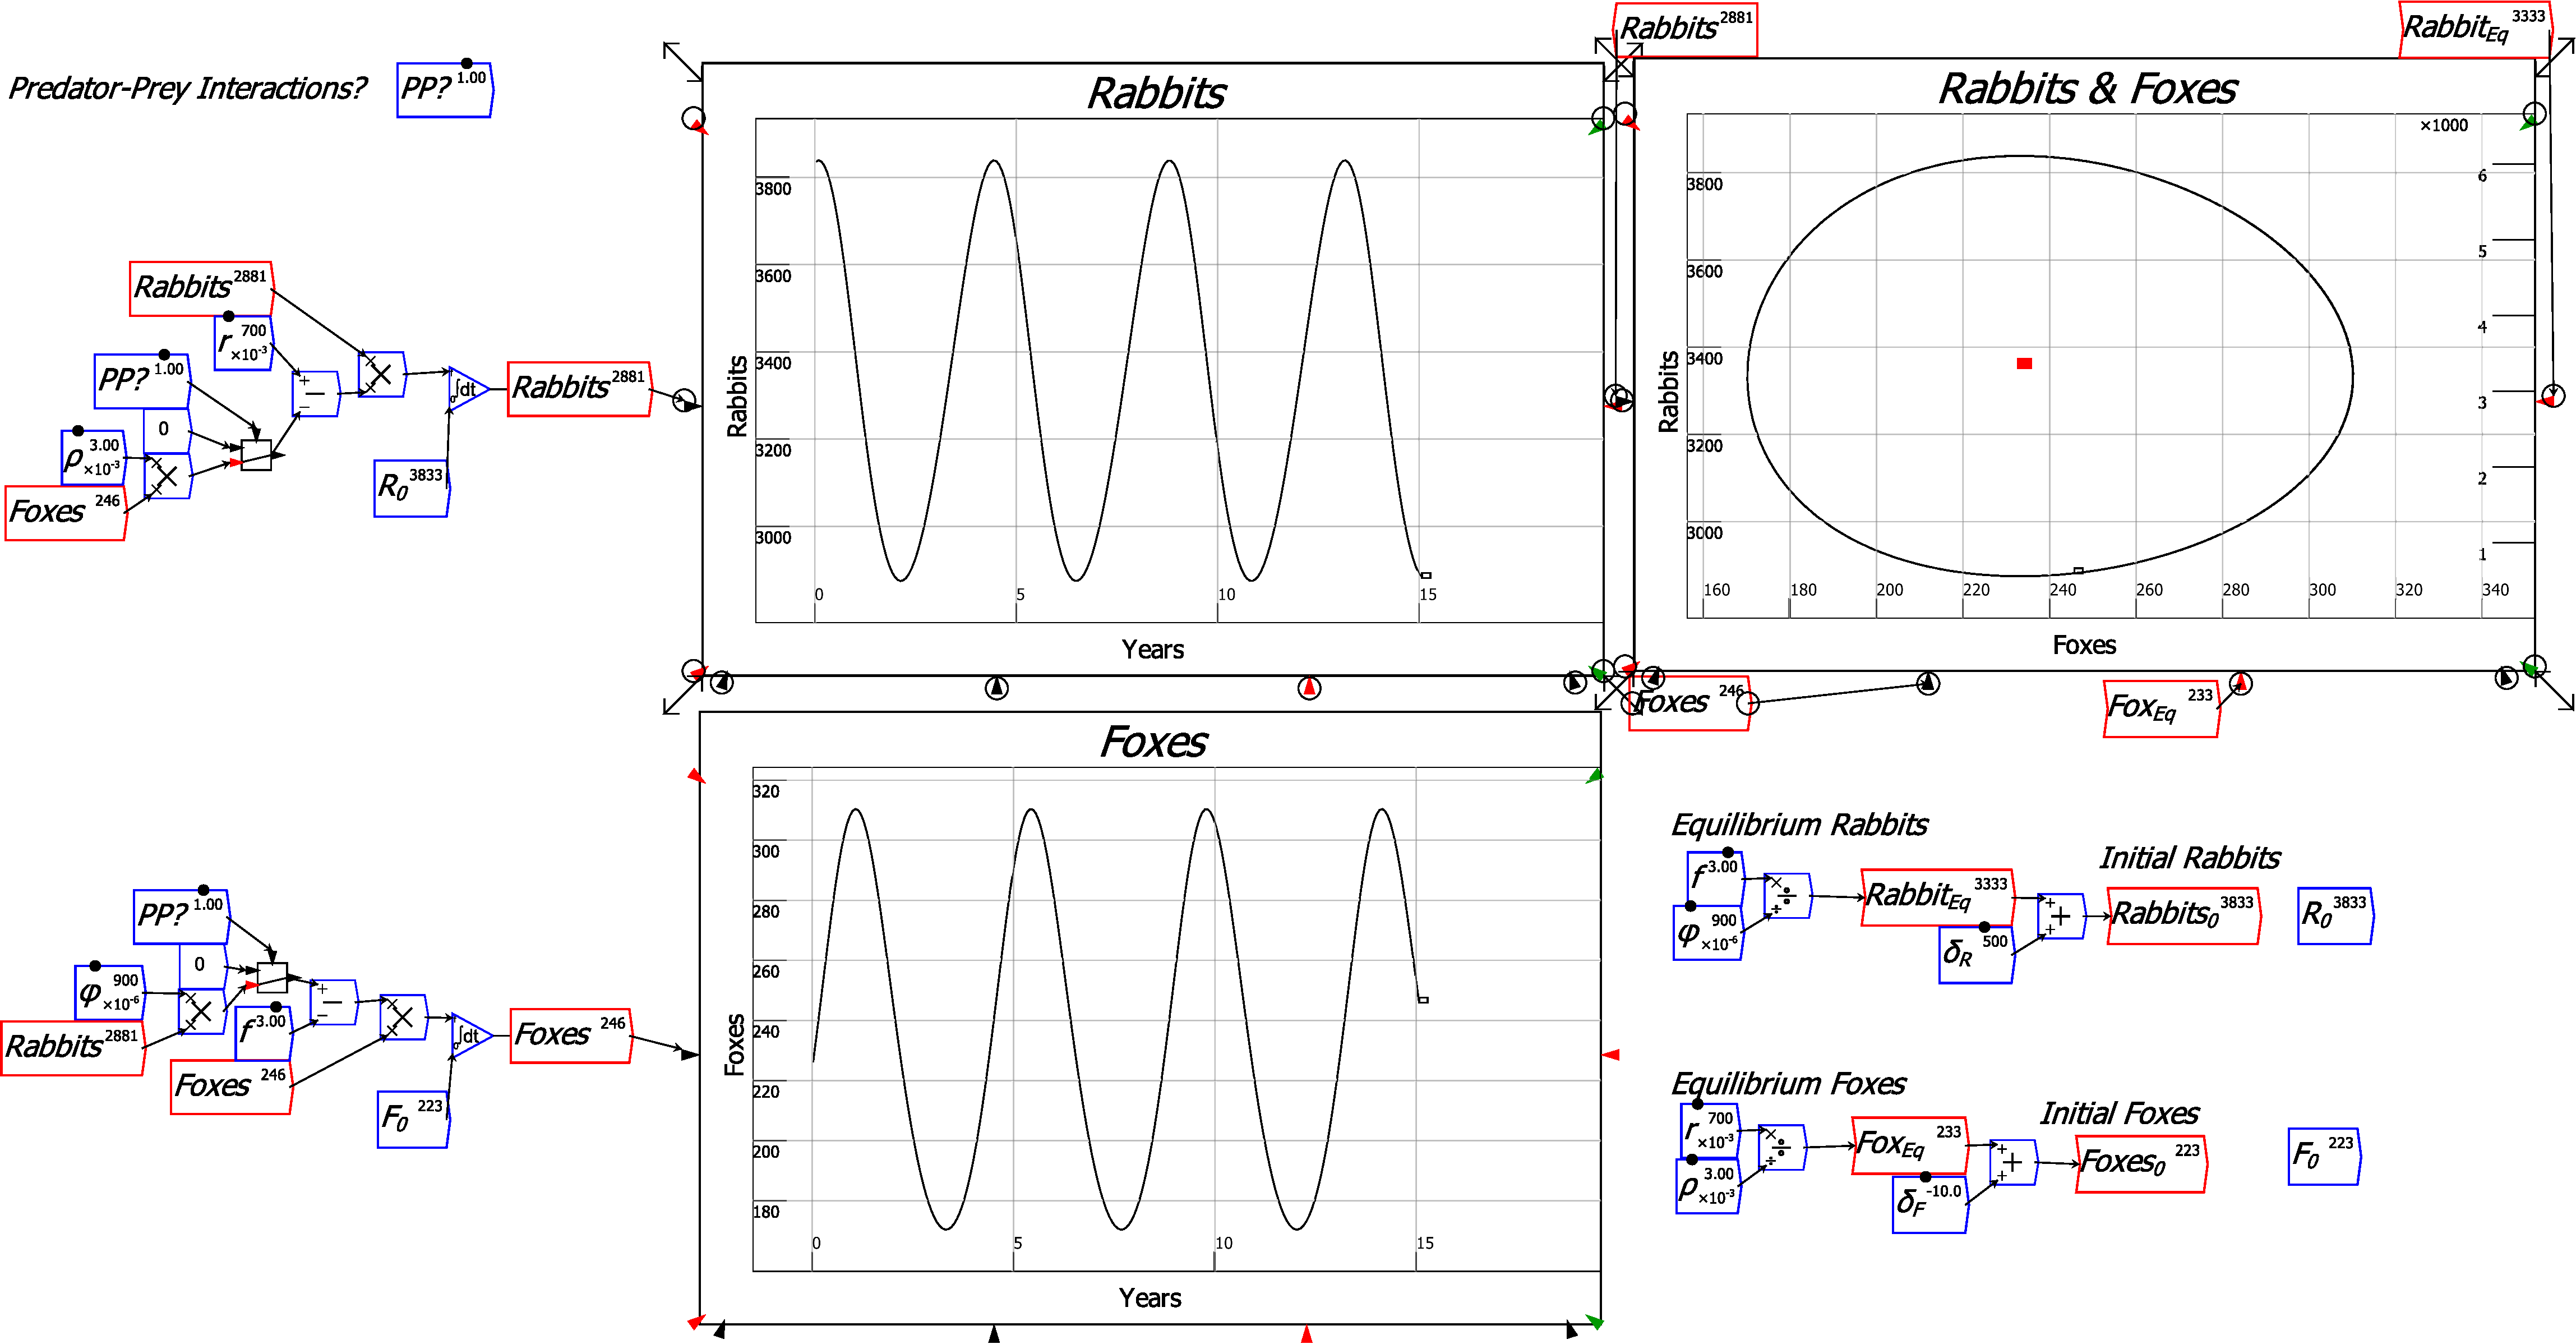
\includegraphics[width=15cm]{images/PredatorPreyRabbitsFoxes}

Programs like Vensim and Simulink have been in existence for decades,
and they are now mature products that provide everything their user-base
of management consultants and engineers want for modeling and analyzing
complex dynamic systems. So why has \emph{Minsky} been developed?
The key reason is its unique feature of Godley Tables \ref{Godley-Tables},
which allow dynamic equations to be developed for monetary transactions
via double-entry bookkeeping tables.

\section{If you are experienced in system dynamics}

\label{intro:experienced-system-dynamics}

As an experienced system dynamics user (or if you've just read \ref{Introduction-Minsky}),
the most important thing you need to know is what \emph{Minsky} provides
that other system dynamics programs do not. That boils down to one
feature: The Godley Table. 

\subsection{Godley Tables}

\label{Godley-Tables}

Godley tables are a unique feature of \emph{Minsky.} They are based
on what could be called the world's first GUI (``Graphical User Interface''),
the accountant's double-entry bookkeeping table.

Double-entry was invented in 15th century Italy \url{https://www.janegleesonwhite.com/double}
to enable accurate recording of financial transactions. The essence
of this method is (a) to classify all of an entity's accounts as either
Assets or Liabilities, with the difference between them representing
the Equity of the entity; and (b) to record every transaction twice,
once as a Credit $\left(CR\right)$and once as a Debit $\left(DR\right)$,
where the definitions of Credit and Debit entries for Assets, Liabilities
and Equity are designed to ensure that the transaction was accurately
recorded. Minsky uses this GUI to generate stock-flow consistent models
of financial flows, but by default uses plus $\left(+\right)$ and
minus $\left(-\right)$ operators (though the accountant's convention
of Credit $\left(CR\right)$and Debit $\left(DR\right)$ can be chosen
via the Options menu). This system guarantees that, no matter how
complex the model is, the equations are internally consistent.

\emph{Minsky} uses this GUI to generate systems of ordinary differential
equations to model financial flows. The columns specify stocks, while
the entries in rows are flows. \emph{The symbolic sum of a column
is thus the rate of change of the associated stock}. \emph{Minsky}
takes a table like the next figure:

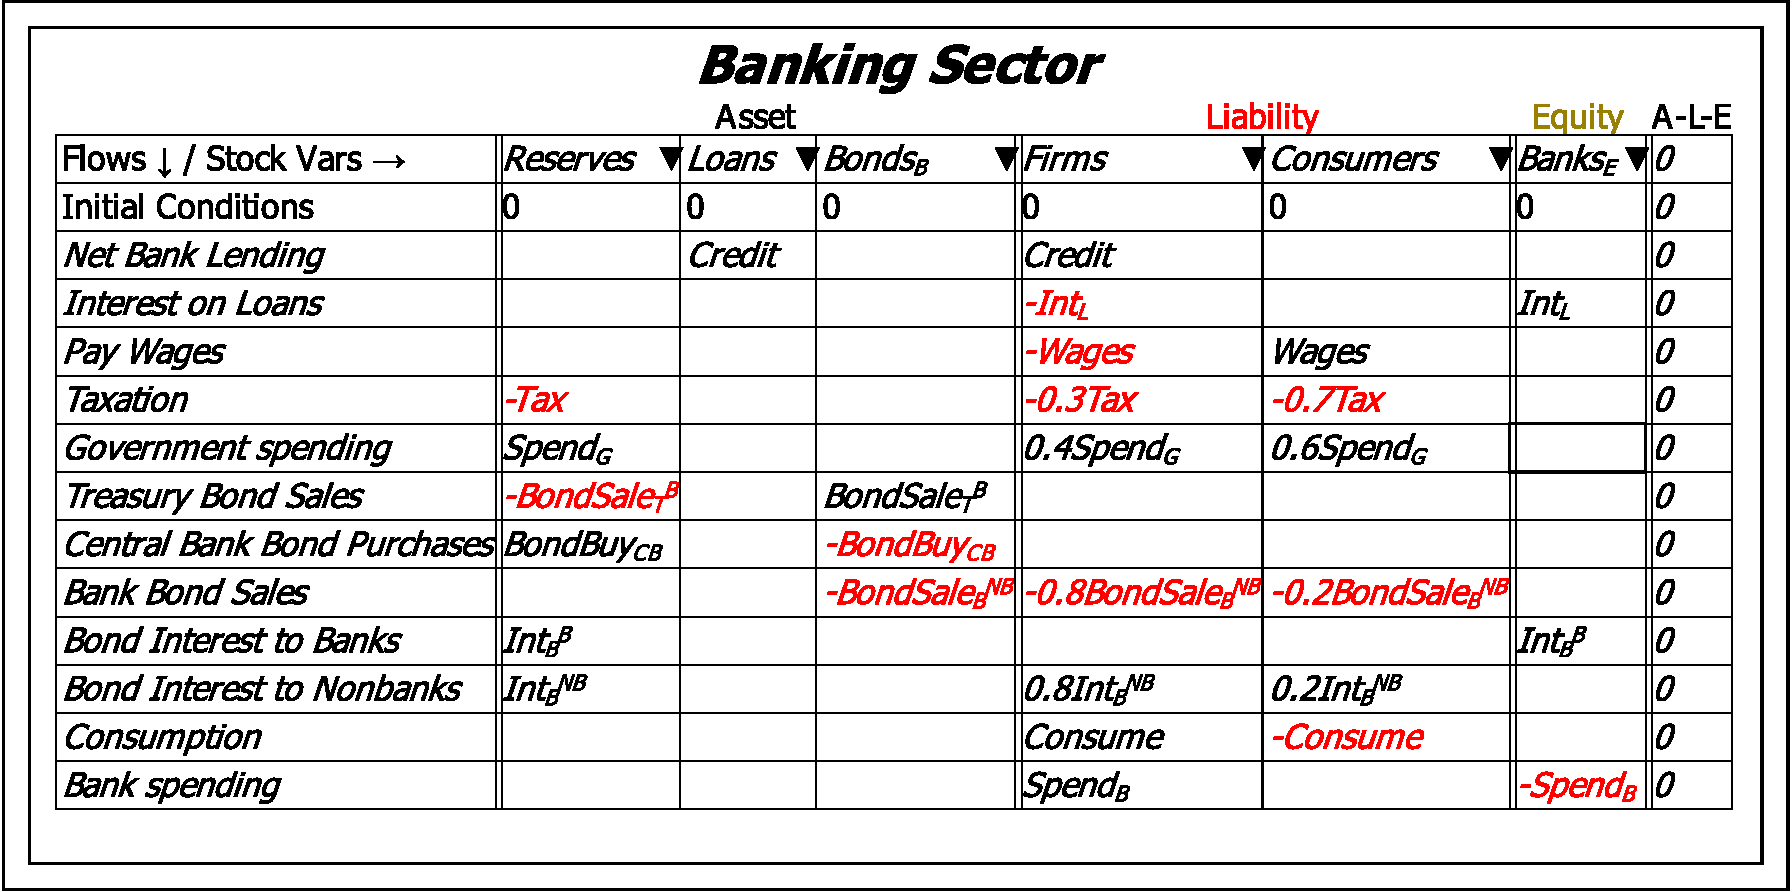
\includegraphics[width=15cm]{images/GodleyTableSingle}

And converts it into a set of dynamic equations, which by construction
are ``stock-flow consistent'':

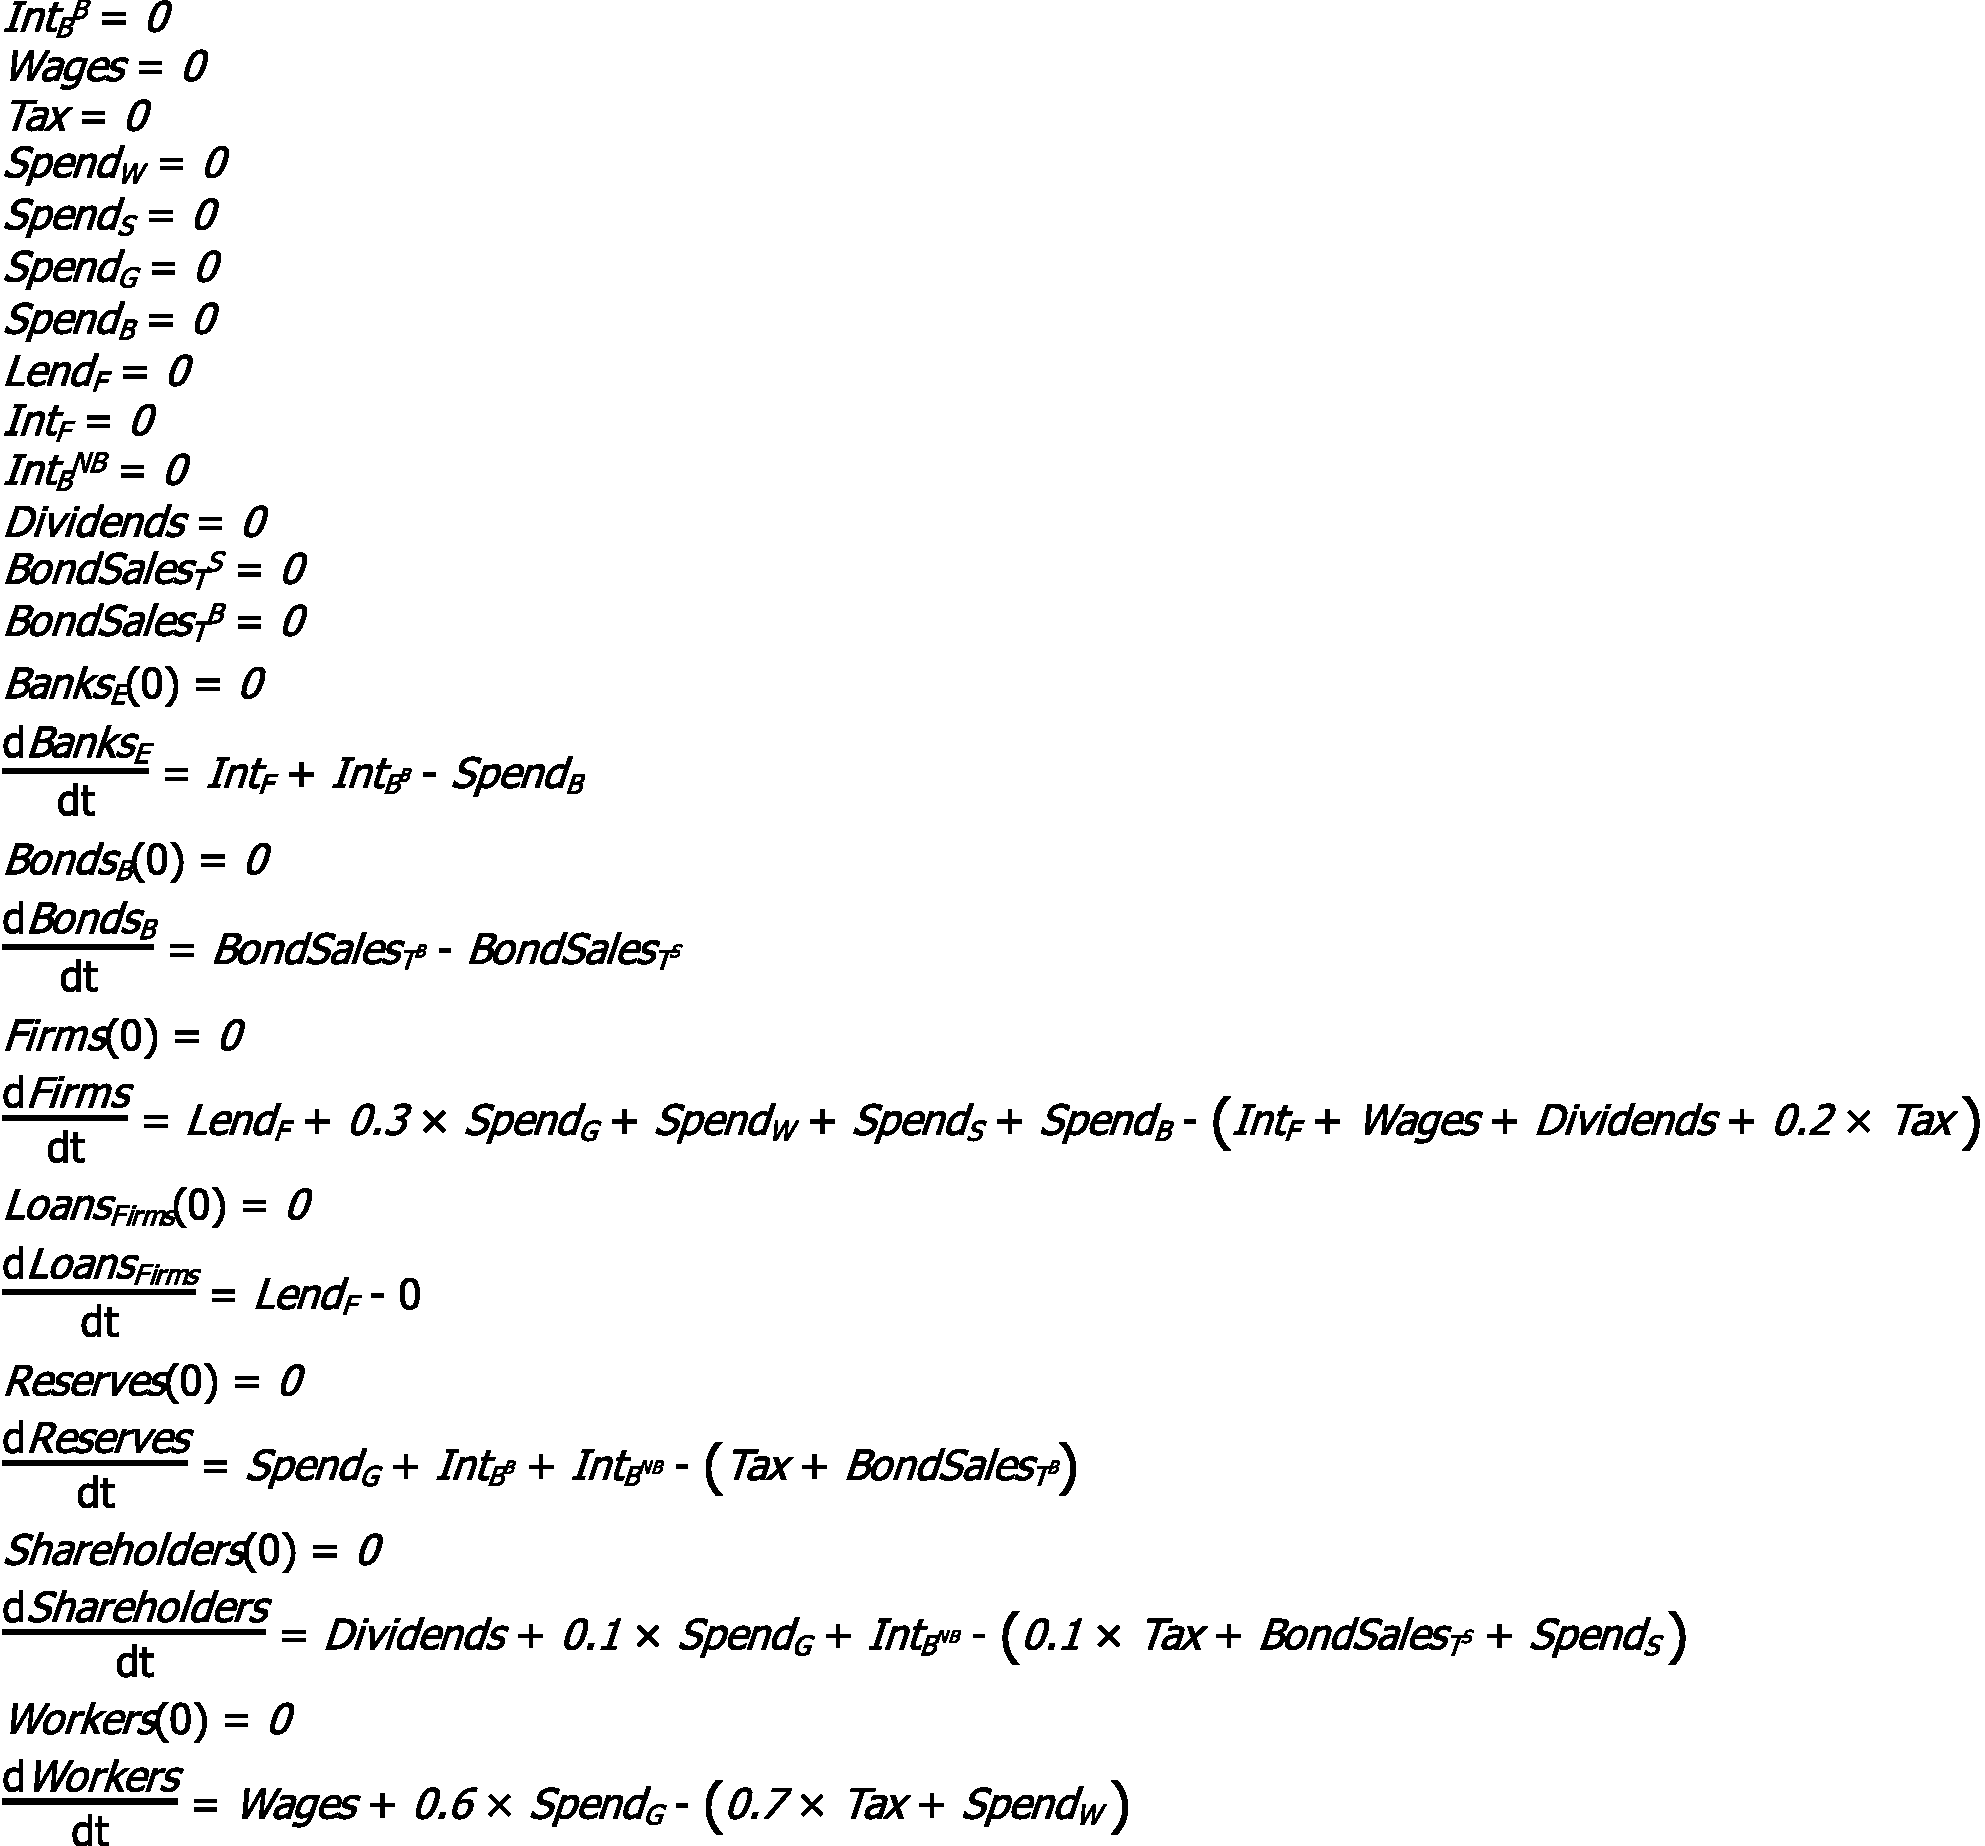
\includegraphics{images/GodleyTableSingleEquations}

The model is completed by defining the flows on the canvas.

In addition, because one entity's financial asset is another's financial
liability, \emph{Minsky} enables the construction of a multi-sectoral
view of financial transactions. The wedge next to every account name
is used on other tables to search for Assets that have not yet been
recorded as a Liability, and vice versa. For example, the previous
Table recorded the financial system from the point of view of the
Banking Sector, for which Reserves---the deposit accounts of private
banks at the Central Bank--are an Asset. Reserves are also a liability
of the Central Bank, and that can be shown in \emph{Minsky} by adding
an additional Godley Table, naming it \emph{Central Bank}, and recording
Reserves as a Liability:

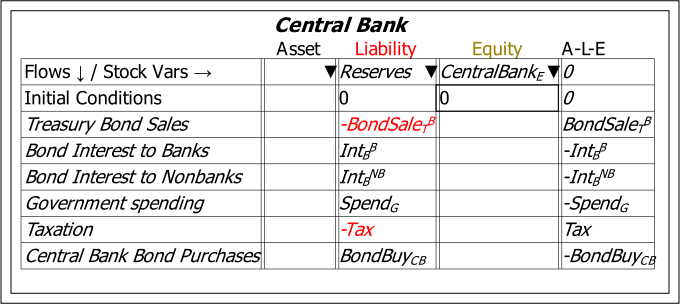
\includegraphics{images/GodleyTableSecondIncomplete}

At this stage, the financial transactions have been entered only once---against
the Central Bank's Liability of Reserves. Each transaction has to
be entered a second time to complete its record, but at present there
are no available accounts in which to record the transactions a second
time.

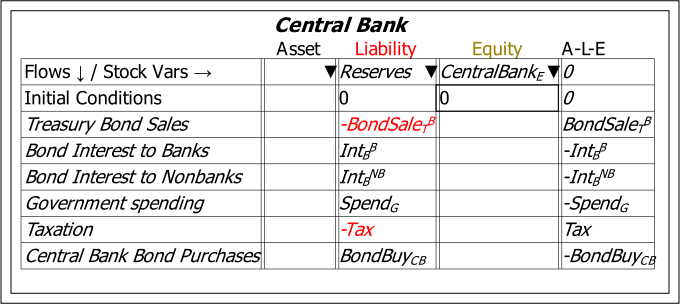
\includegraphics{images/GodleyTableSecondIncomplete}

Bond purchases by the Central Bank indicate the need for to show bonds
owned by the Central Bank as an asset, while the other transactions
indicate the need to show the Treasury's account at the Central Bank,
the ``Consolidated Revenue Fund'', as an additional liability:

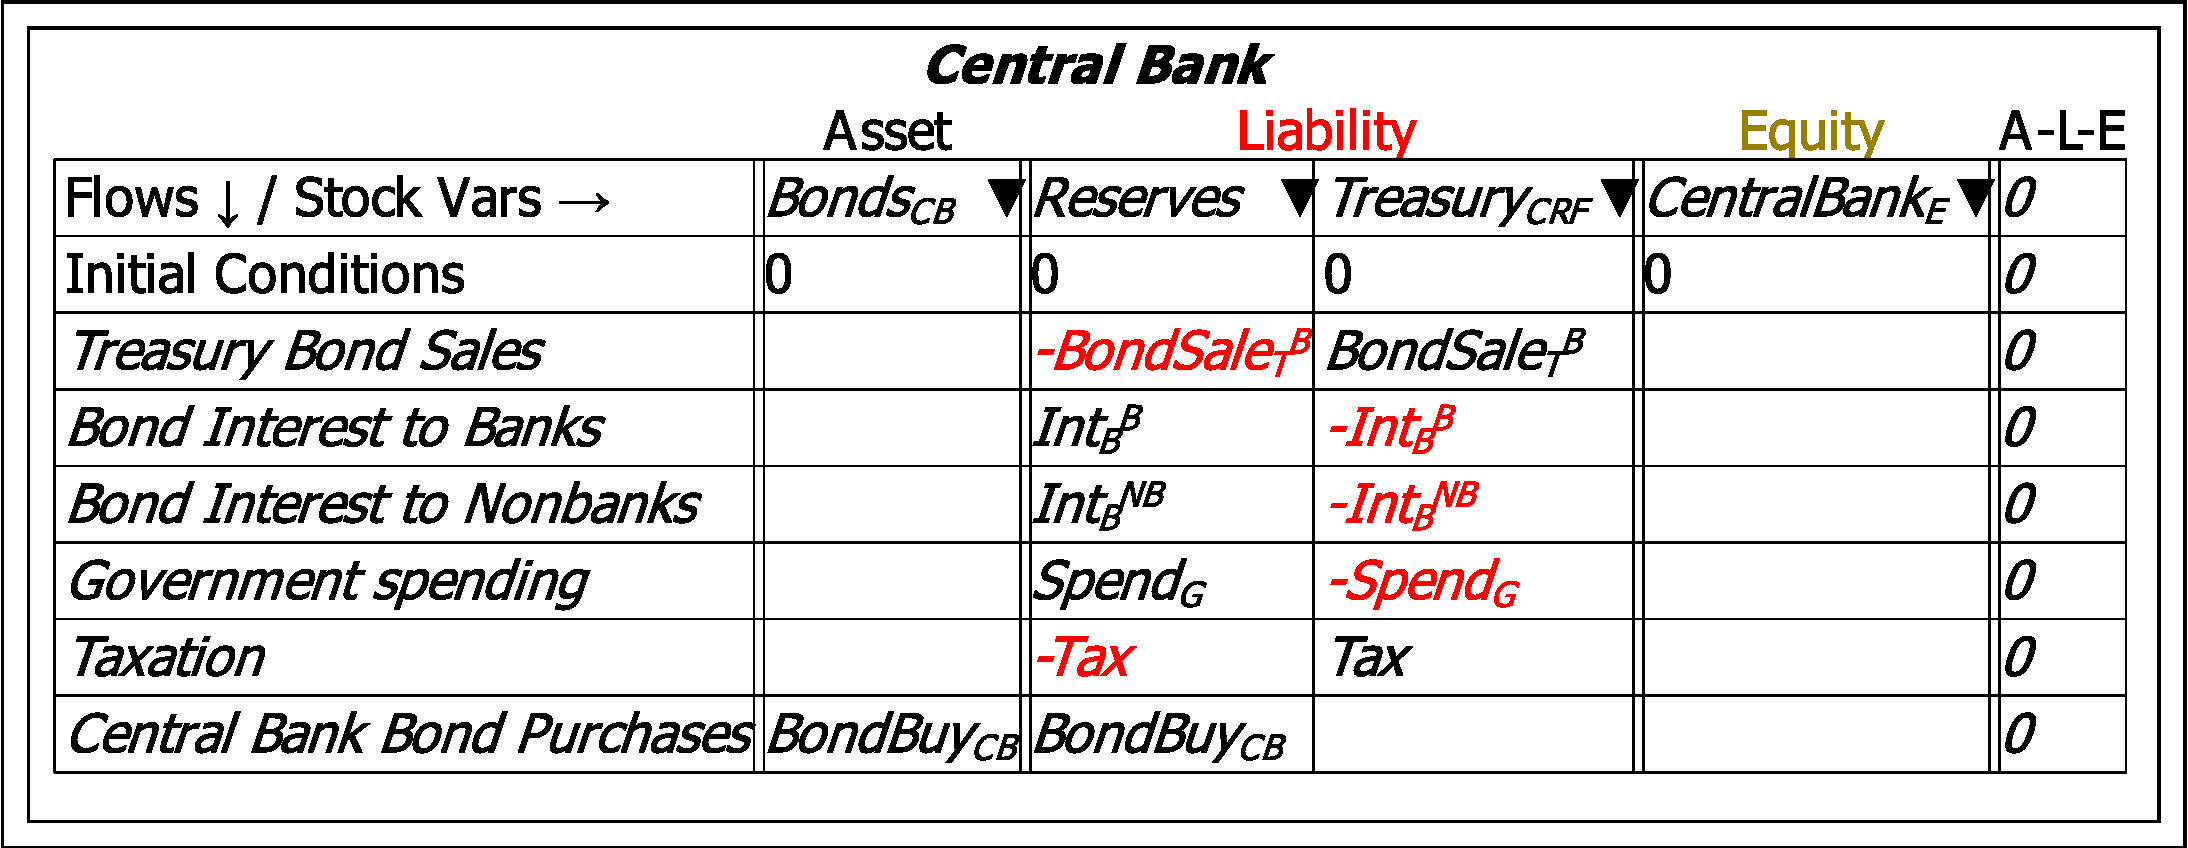
\includegraphics{images/GodleyTableSecondComplete}

This is an inherently better way to generate a dynamic model of financial
flows than the flowchart method used by all other system dynamics
programs, for at least four reasons: 
\begin{itemize}
\item All financial transactions are flows between entities. The tabular
layout captures this in a very natural way: each row shows where a
flow originates, and where it ends up;
\item The program imposes the rules of double-entry bookkeeping, in which
entries on each row balance to zero according to the {\em accounting
equation} $(Assets=Liabilities+Equity)$. If you don't ensure that
each flow starts somewhere and ends somewhere, then the program will
identify your mistake;
\item The double-entry perspective assists in the completion of a model,
since the requirement of a matching entry for each transaction indicates
the accounts that are needed to complete the accounting; and
\item Double-entry bookkeeping acts as a prohibition against recording invalid
transactions.
\end{itemize}
\emph{Minsky} thus adds an element to the system dynamics toolkit
which is essential for modeling the monetary flows that are an intrinsic
aspect of a market economy.

\subsection{\emph{Minsky}'s unusual system dynamics features}

\emph{Minsky} differs from conventional system dynamics models in
various ways:
\begin{itemize}
\item Most programs store their mathematical formulas within a text block,
which must be opened to see its equation. The mathematics of a \emph{Minsky}
model is shown explicitly on the design canvas;
\item Most programs require every entity used to build an equation to be
wired to the block in which the equation is defined, while each entity
is shown only once on the design canvas. This generates the familiar
system dynamics ``spaghetti diagram'', as even practitioners---rather
than merely critics---often describe their models. \emph{Minsky}
enables entities to be shown multiple times on the design canvas,
which substantially reduces the number of wires needed to build a
model. \emph{Minsky}'s equations therefore resemble small ``spider
webs'', rather than large bowls of spaghetti. This makes it easier
to understand what a model does; and
\item Most programs show the end results of a simulation. \emph{Minsky}
shows simulations dynamically, and the numerical values of parameters
and variables are shown on the parameters and variables themselves.
Parameters can be altered during a simulation, which enables them
to be used as a ``control panel'' for simulation of policy proposals,
etc.
\end{itemize}
These unusual features are best illustrated by building a simple model
in \emph{Minsky}. The next section explains how to build a simpler
version of the predator-prey model shown in \ref{intro:new-system-dynamics}.

\subsection{Building a predator-prey model in Minsky}

\label{Minsky model building}

The first step in building the Rabbits and Foxes model in \emph{Minsky}
is to insert two integral blocks on the canvas---one for Rabbits
and the other for Foxes. An integral block is inserted by clicking
on the 
\includegraphics{images/integral} operator \ref{Variable:integral}.
To alter its name from the generic ``int1'', either double-click
on the widget, which brings up the context menu for integral blocks,
or hover the mouse over the block and click the right-mouse button,
and choose ``Edit'' to bring up the edit form (another method is
to choose ``Rename all instances'' from the context menu). Name
the two variables Rabbits and Foxes respectively, and you will have
the following objects on your canvas:

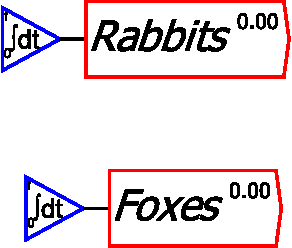
\includegraphics{images/PredatorPreyRabbitsFoxesIntegralsOnly}

As is typical of dynamic models, the rates of change of the variables
Rabbits and Foxes depends on their current values. You therefore need
to copy the variable names, which you do using the context menu command
``Copy item''. Do this and place both on the canvas:

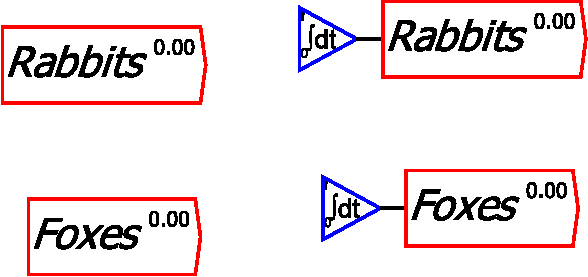
\includegraphics{images/PredatorPreyRabbitsFoxes02}

Next add the parameters that determine the rates of growth and death
of the two species. The non-zero equilibrium is set by the zeros of
$\left(r-\rho\times Foxes\right)$ and $\left(-f+\phi\times Rabbits\right)$.

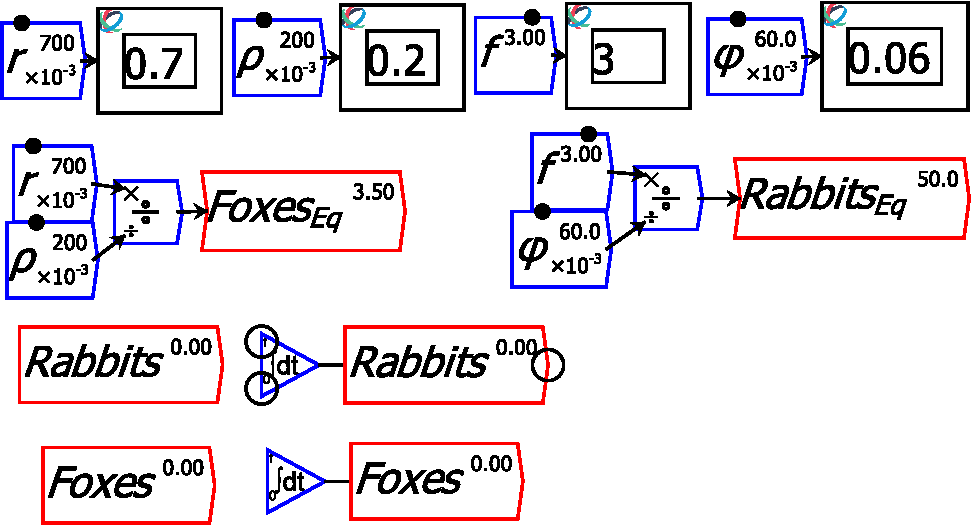
\includegraphics{images/PredatorPreyRabbitsFoxes03ParametersAdded}

Finally, the equations for the rates of growth of the two species
are wired up, and the model can be simulated.

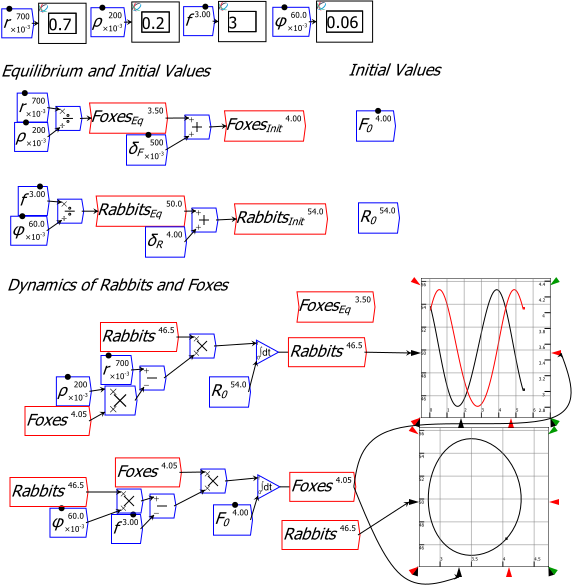
\includegraphics{images/PredatorPreyRabbitsFoxes04Equations}

If you don't want to display the complete equations on the canvas,
you can use grouping to hide the complexity. The next figure illustrates
several ways to use groups, and the feature that groups become transparent
(and can be edited \emph{in situ}) as the zoom level increases.

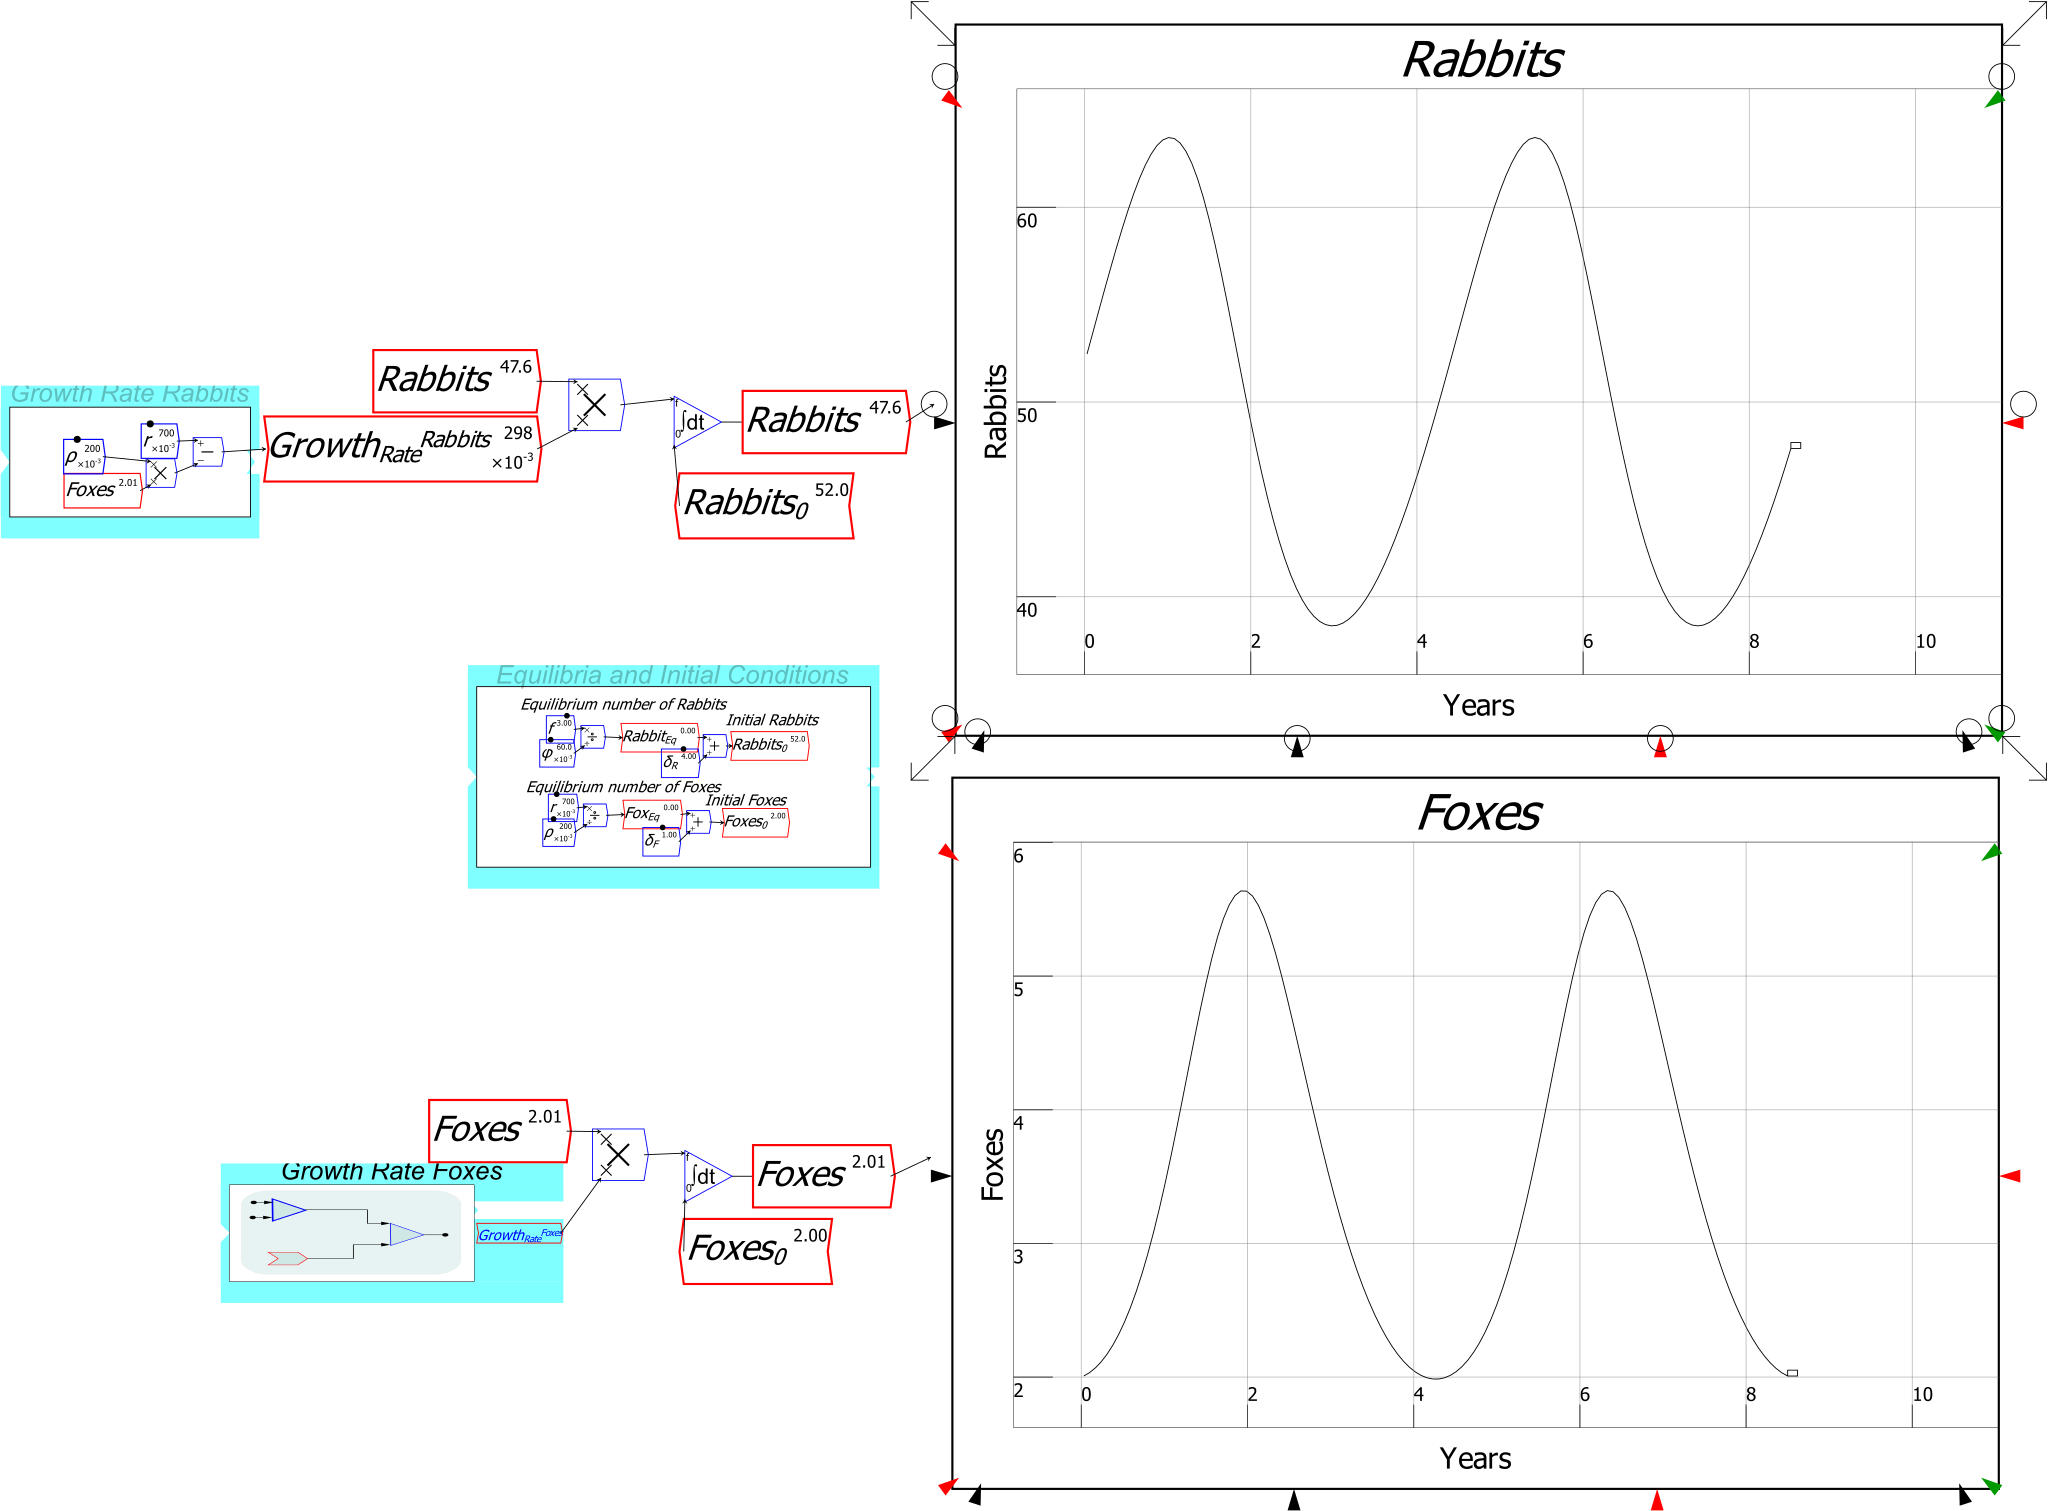
\includegraphics[width=15cm]{images/PredatorPreyRabbitsFoxes05Grouping}

\subsection{Building monetary models in \emph{Minsky}}

Monetary models are actually simpler to build in \emph{Minsky} than
block diagram models, because all you have to do is to name the accounts
in the Godley Table, and then define the flows on the canvas. \emph{Minsky}
automatically generates the differential equations for you.

Building the model starts with placing a Godley Table on the canvas
by clicking on the Godley Table operator 
\includegraphics{images/GodleyIcon}.
The figure below shows a single Godley Table on the canvas, which
has been labelled ``Banking Sector'' using the context menu ``Title''
command.


\includegraphics{images/MonetaryModel01GodleyTable01}

Next either double-click on the icon, or choose ``Open Godley Table''
from the context menu, to bring up the Godley Table form:

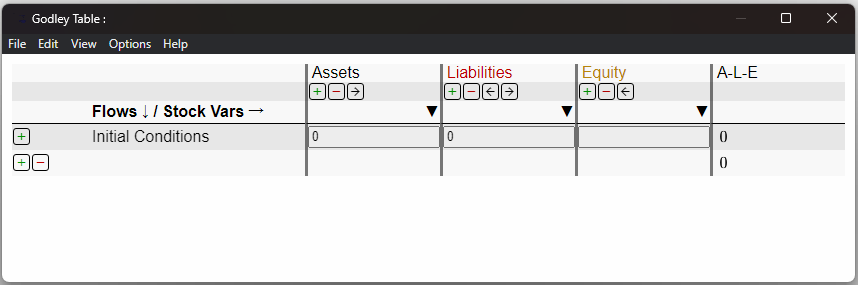
\includegraphics{images/GodleyTableEditWindow}

We'll build a model of private money creation in this first example.

\subsubsection{Modelling private money creation}

Add four Stocks to this table: \emph{Reserves }and \emph{Loans} as
Assets, \emph{Deposits} as a Liability, and \emph{Banks}\textsubscript{\emph{Equity}}
as the Equity of the Banks (type Banks\_\{Equity\} to subscript the
word Equity). Go back to the Design canvas and choose ``Editor mode''
from the context menu, and you will see the table displayed as follows
(you will need to resize the table using the Resizing arrows, which
are visible when your mouse is hovering over the table)

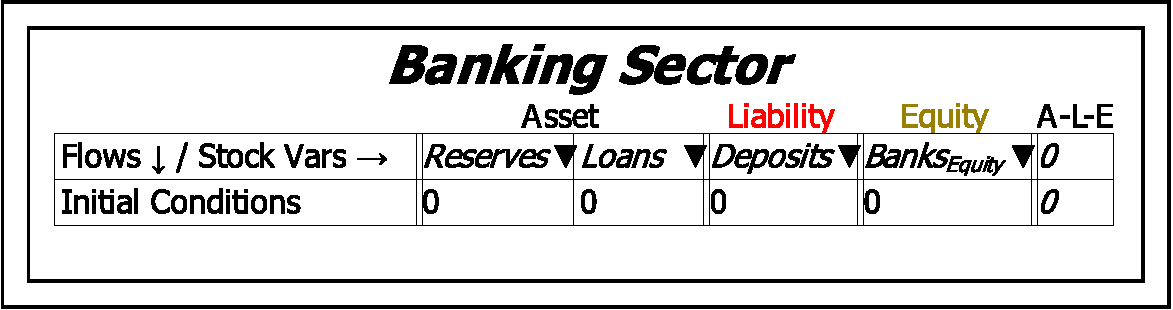
\includegraphics{images/MonetaryModel01GodleyTable02}

Now enter numbers into the ``Initial Conditions'' row. Put 90 in
\emph{Reserves}, 10 in \emph{Loans}, 80 in \emph{Deposits}, and 20
in \emph{BanksEquity}. 

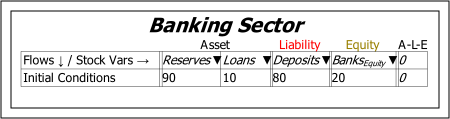
\includegraphics{images/MonetaryModel01GodleyTable03InitialConditions}

Then add three flows to the model: Net Bank Loans (which can be negative
if people in the aggregate are paying their debts down rather than
taking on new debt), Interest Payments, and Bank Spending. Call Net
Bank Loans ``Credit'', Interest Payments ``Interest\_L'' (the
subscript is to distinguish interest on loans from interest on bonds,
which we'll introduce later), and Bank Spending ``Spend\_B'' (the
subscript is to distinguish Bank Spending from Government Spending,which
we'll introduce later).

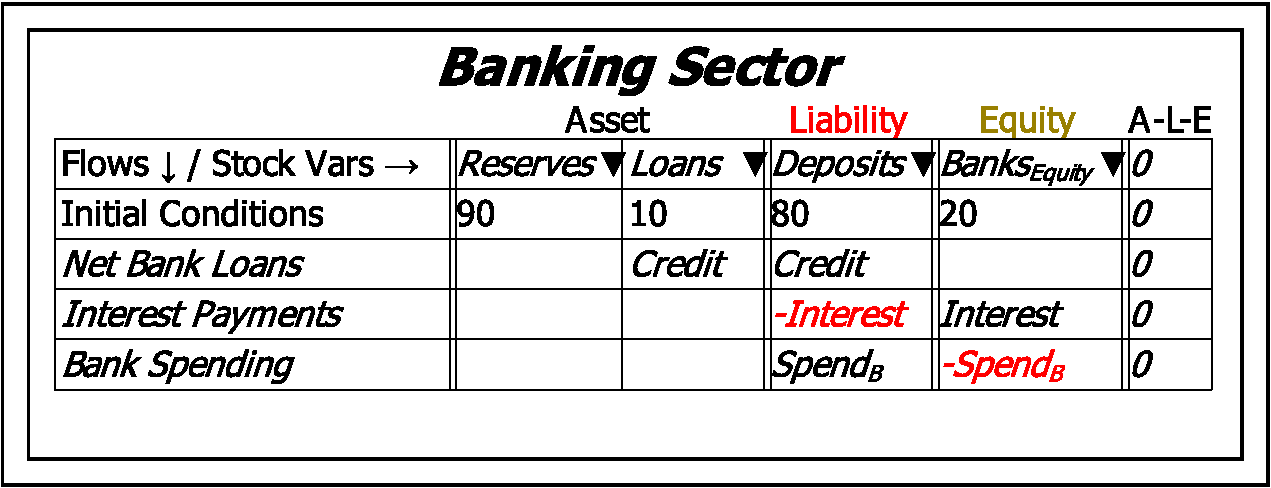
\includegraphics{images/MonetaryModel01GodleyTable04AddFlows}

Next, return to the canvas and use the Godley Table context menu commands
\emph{Copy flow variables} and \emph{Copy stock variables} to copy
all flows and stocks and place them on the canvas, where they can
be defined.

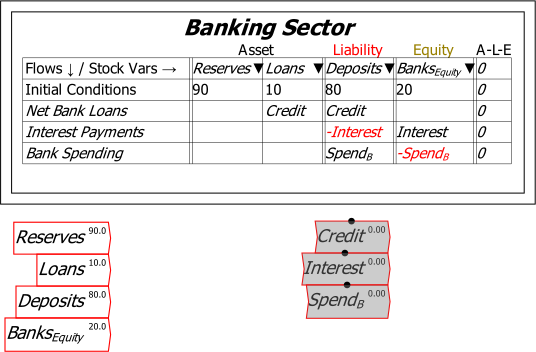
\includegraphics{images/MonetaryModel01GodleyTable05DefineFlows01}

The easiest flow to define is \emph{Interest}, since this is the rate
of interest times \emph{Loans}. To define this, first define the parameter
\emph{Int}\textsubscript{\emph{Rate}}\emph{}\textsuperscript{\emph{Loans}}:
just type Int\_\{Rate\}\textasciicircum\{Loans\} on the canvas and,
once you've finished entering the text, the Variable/Parameter definition
form will appear. Put 0.05 as the Initial Value, 0.2 as the \emph{Slide
Bounds: Max}, 0.02 as the \emph{Min}, and 0.01 as the \emph{Slider
Step Size}.

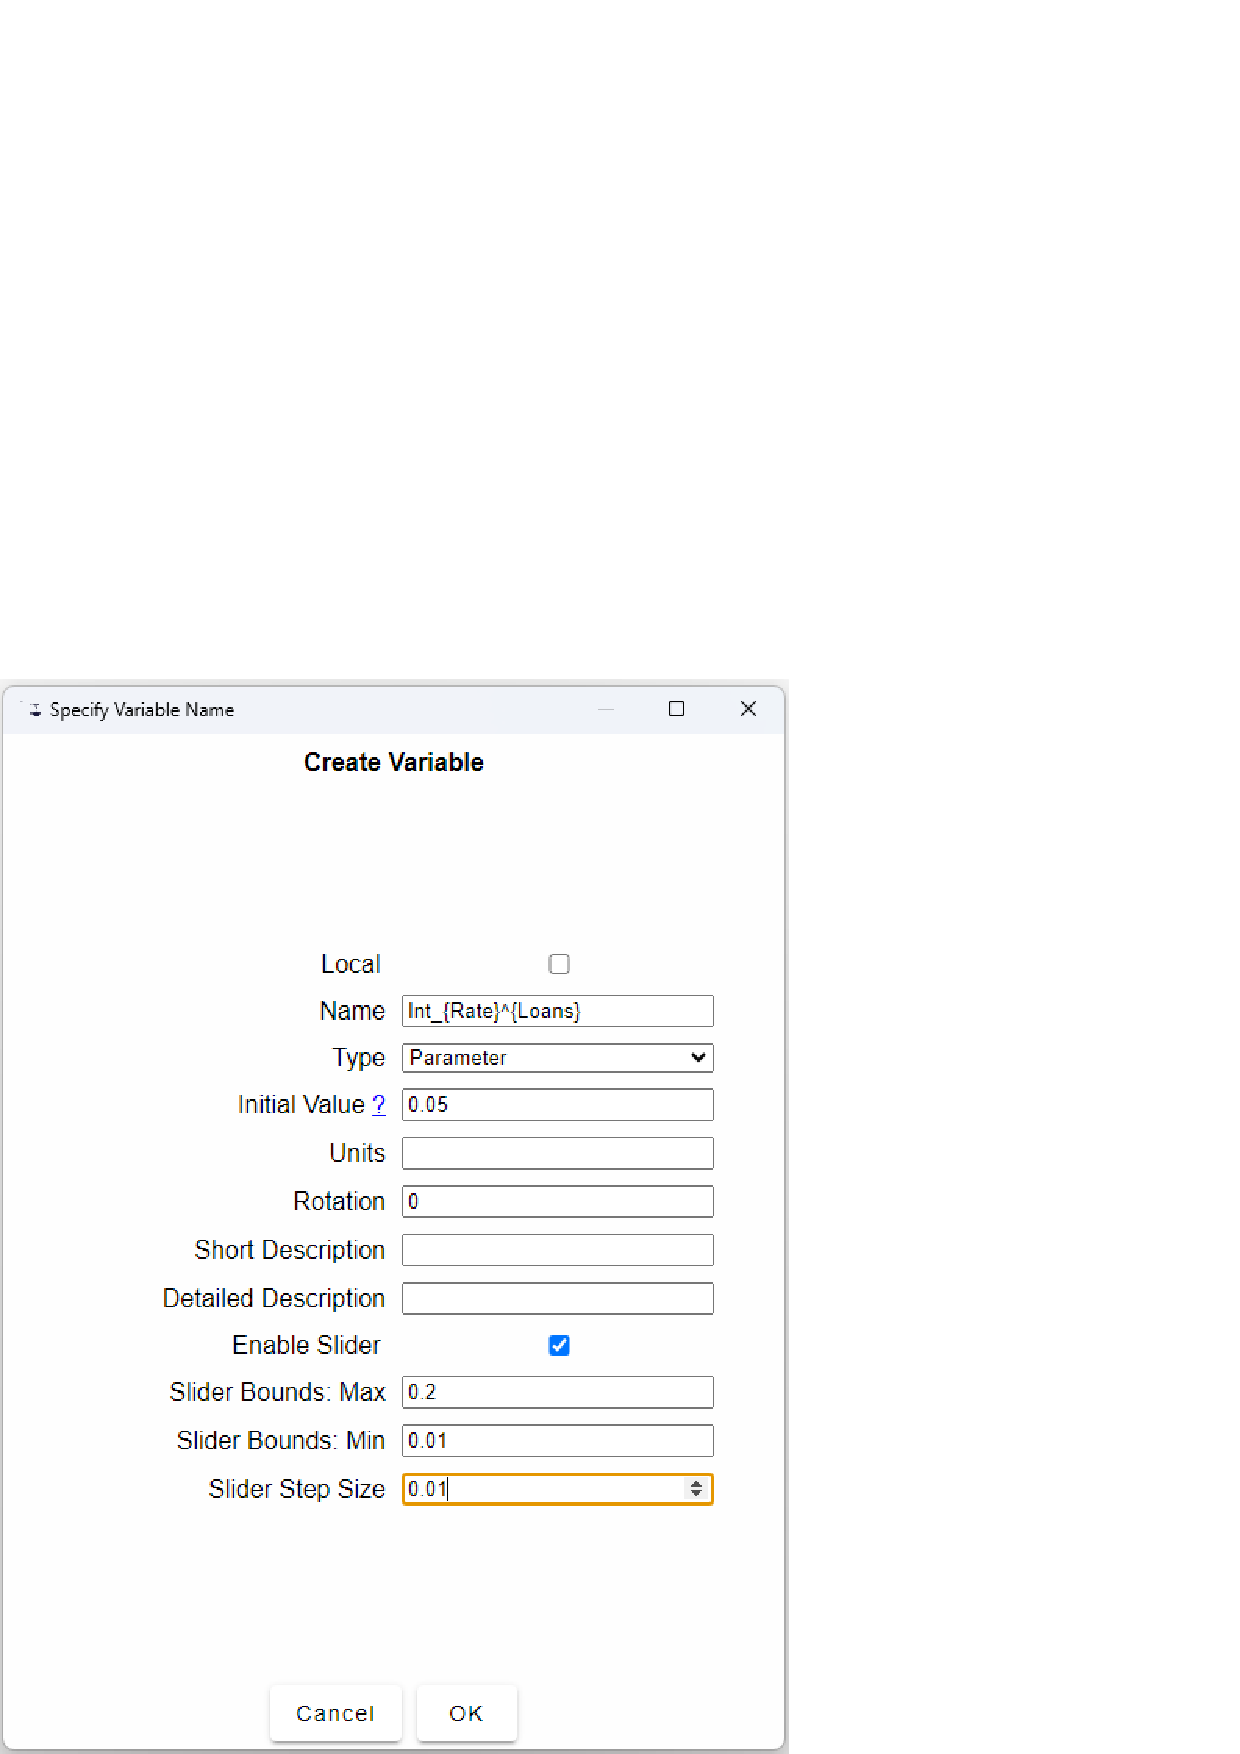
\includegraphics{images/MonetaryModel01GodleyTable05DefineFlows03}

Wire this parameter and \emph{Loans }up to a multiply block 
\includegraphics{images/multiply}\ref{Operation:multiply}
and attach it to the flow Interest, and you have defined the first
of three flows in this extremely simple model.

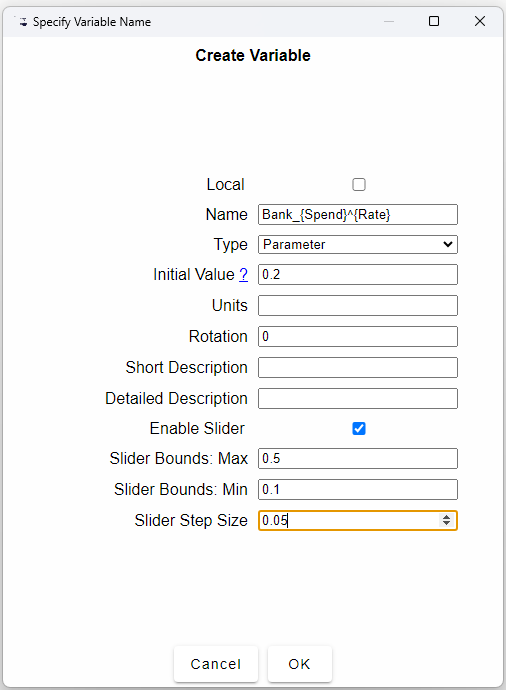
\includegraphics{images/MonetaryModel01GodleyTable05DefineFlows04}

Now define \emph{Spend}\textsubscript{\emph{B}} as a multiple \emph{Bank}\textsubscript{\emph{Spend}}\emph{}\textsuperscript{\emph{Rate}}
of the \emph{Banks}\textsubscript{\emph{Equity}}. Give the parameter
a small Initial Value---say 0.2---which means that Banks spend 20\%
of their equity into the economy every year---this represents paying
dividends, wages and bonuses to households, buying goods and services
off firms, etc. Set Max to 0.5, Min to 0.1, and the Step Size to 0.05.

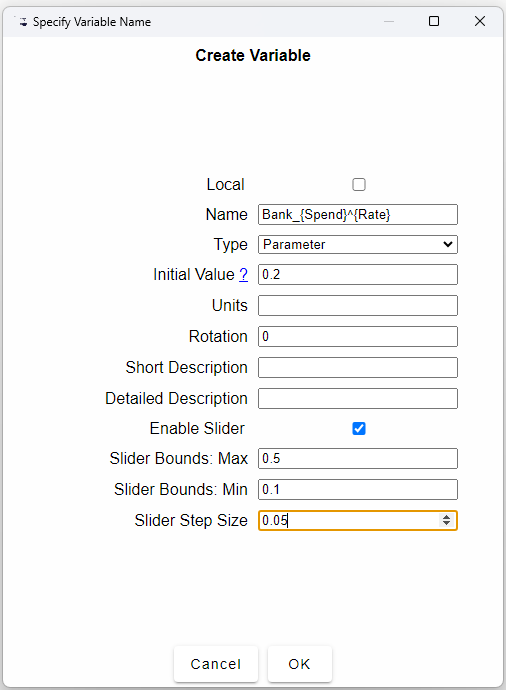
\includegraphics{images/MonetaryModel01GodleyTable05DefineFlows04}

Your canvas should now look like this:

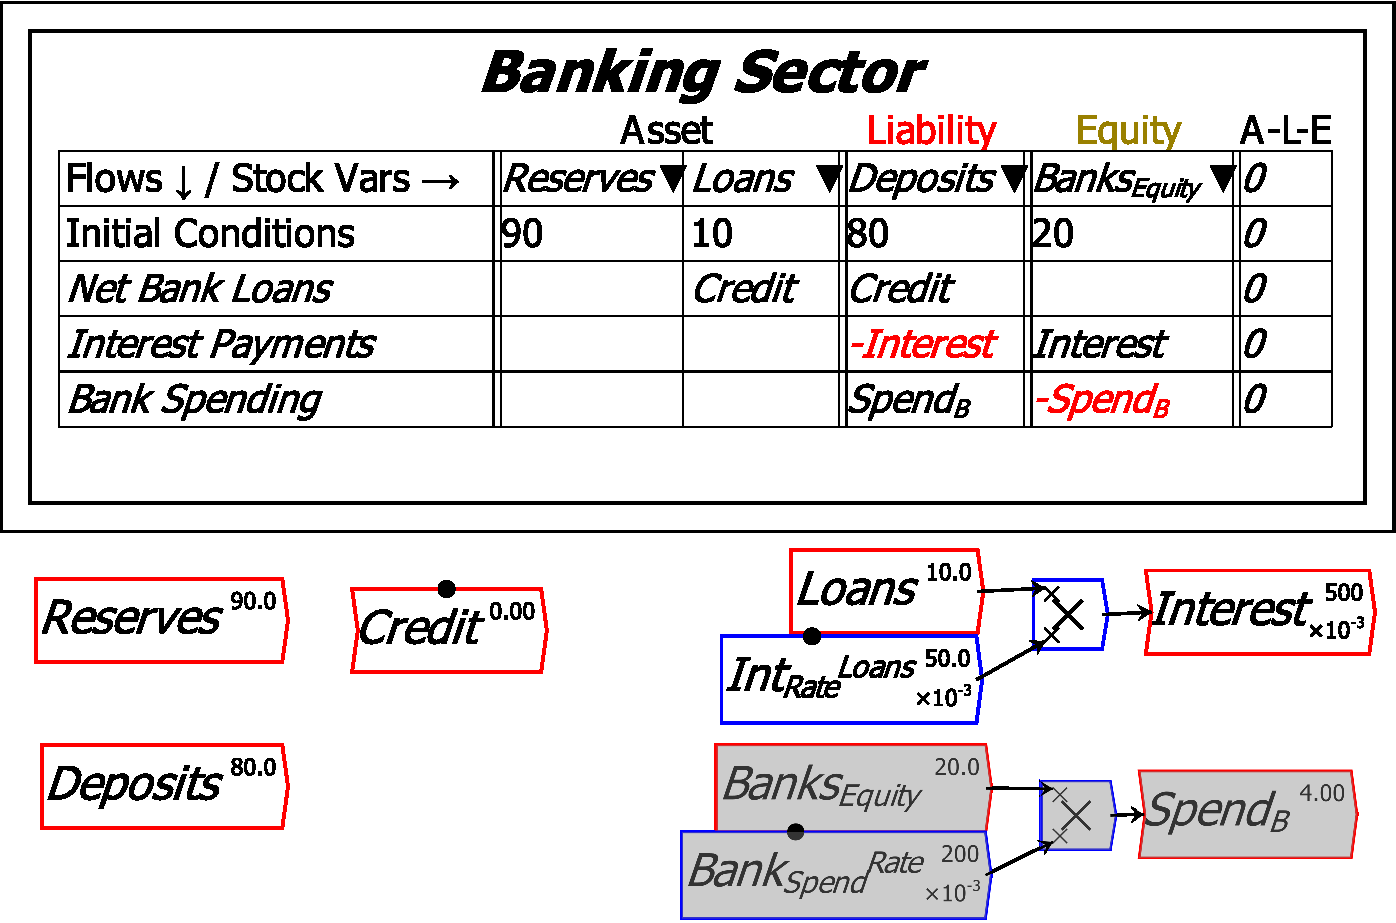
\includegraphics{images/MonetaryModel01GodleyTable05DefineFlows05}

This is sufficient to build a model of just financial stocks and flows,
if you edit \emph{Credit} to give it a Max, Min and Step Size in keeping
with the other magnitudes in the model--say a Max of 10, Min of -10,
and Step Size of 1. Add two Plots 
\includegraphics{images/plotWidget}\ref{PlotWidget},
one for Stocks and one for Flows, attach the Stocks and Flows to their
inputs, put a copy of \emph{Credit} at the top of the model for ease
of access, click on the Run button \textifsymbol[ifgeo]{100}, and
vary the value of \emph{Credit }to see what happens:

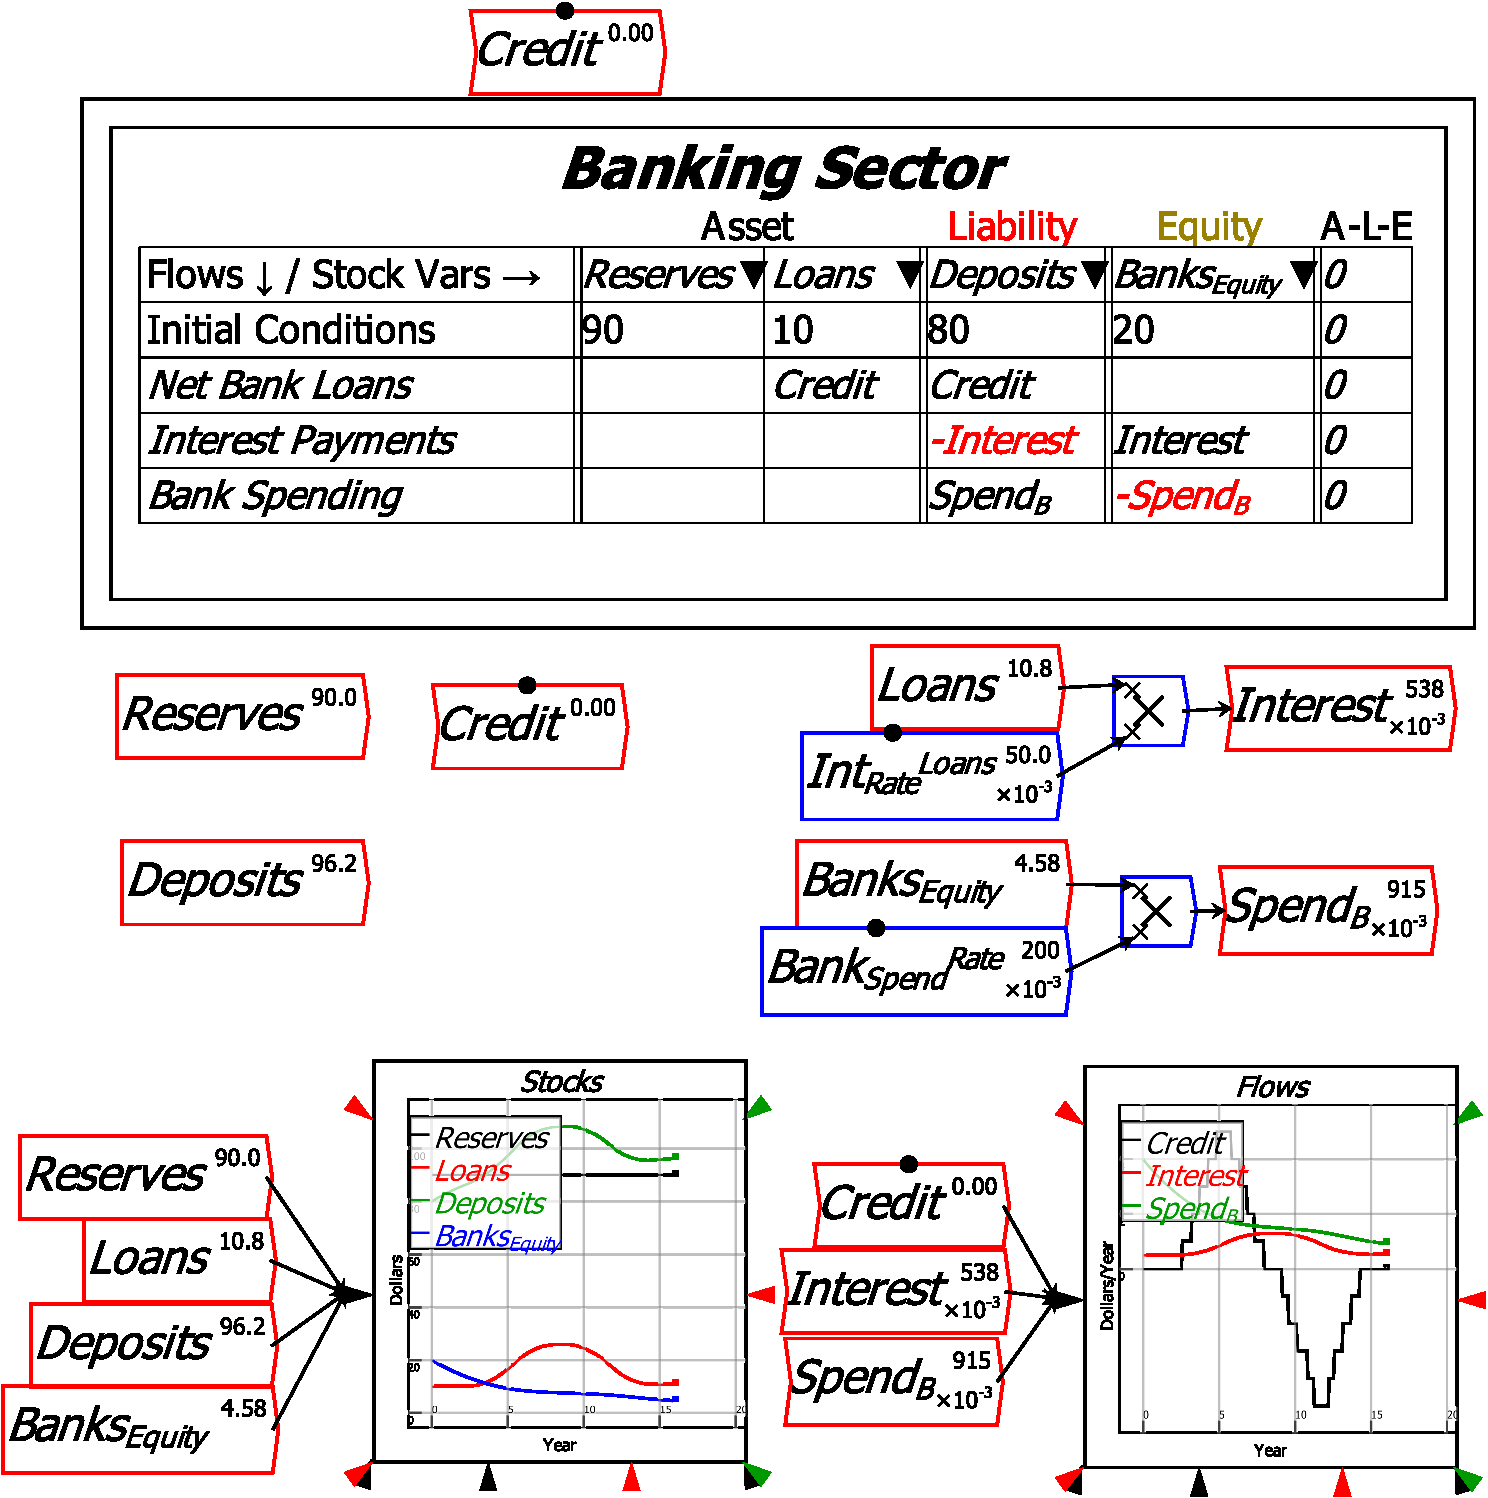
\includegraphics{images/MonetaryModel01GodleyTable06Simulate01}

To link this very simple model to economic concepts, make the ``Friedmanite''
assumption that GDP equals Money times Velocity. Define Money as the
sum of Deposits plus \emph{Banks}\textsubscript{\emph{Equity}},
and define \emph{Velocity} as a parameter with an Initial Value of
2, Max of 4, Min of 0.5, and Step Size of 0.1. Define a parameter
\emph{Credit}\textsubscript{\emph{Ratio}} and give it an Initial
Value of 0, Max of 0.1, Min of minus 0.1, and Step Size of 0.01. Also
define the percentage growth rate as the differential of GDP divided
by itself and put through a percentage operator. Run the model and
vary \emph{Credit}\textsubscript{\emph{Ratio}} using the arrow keys
as you run a simulation.

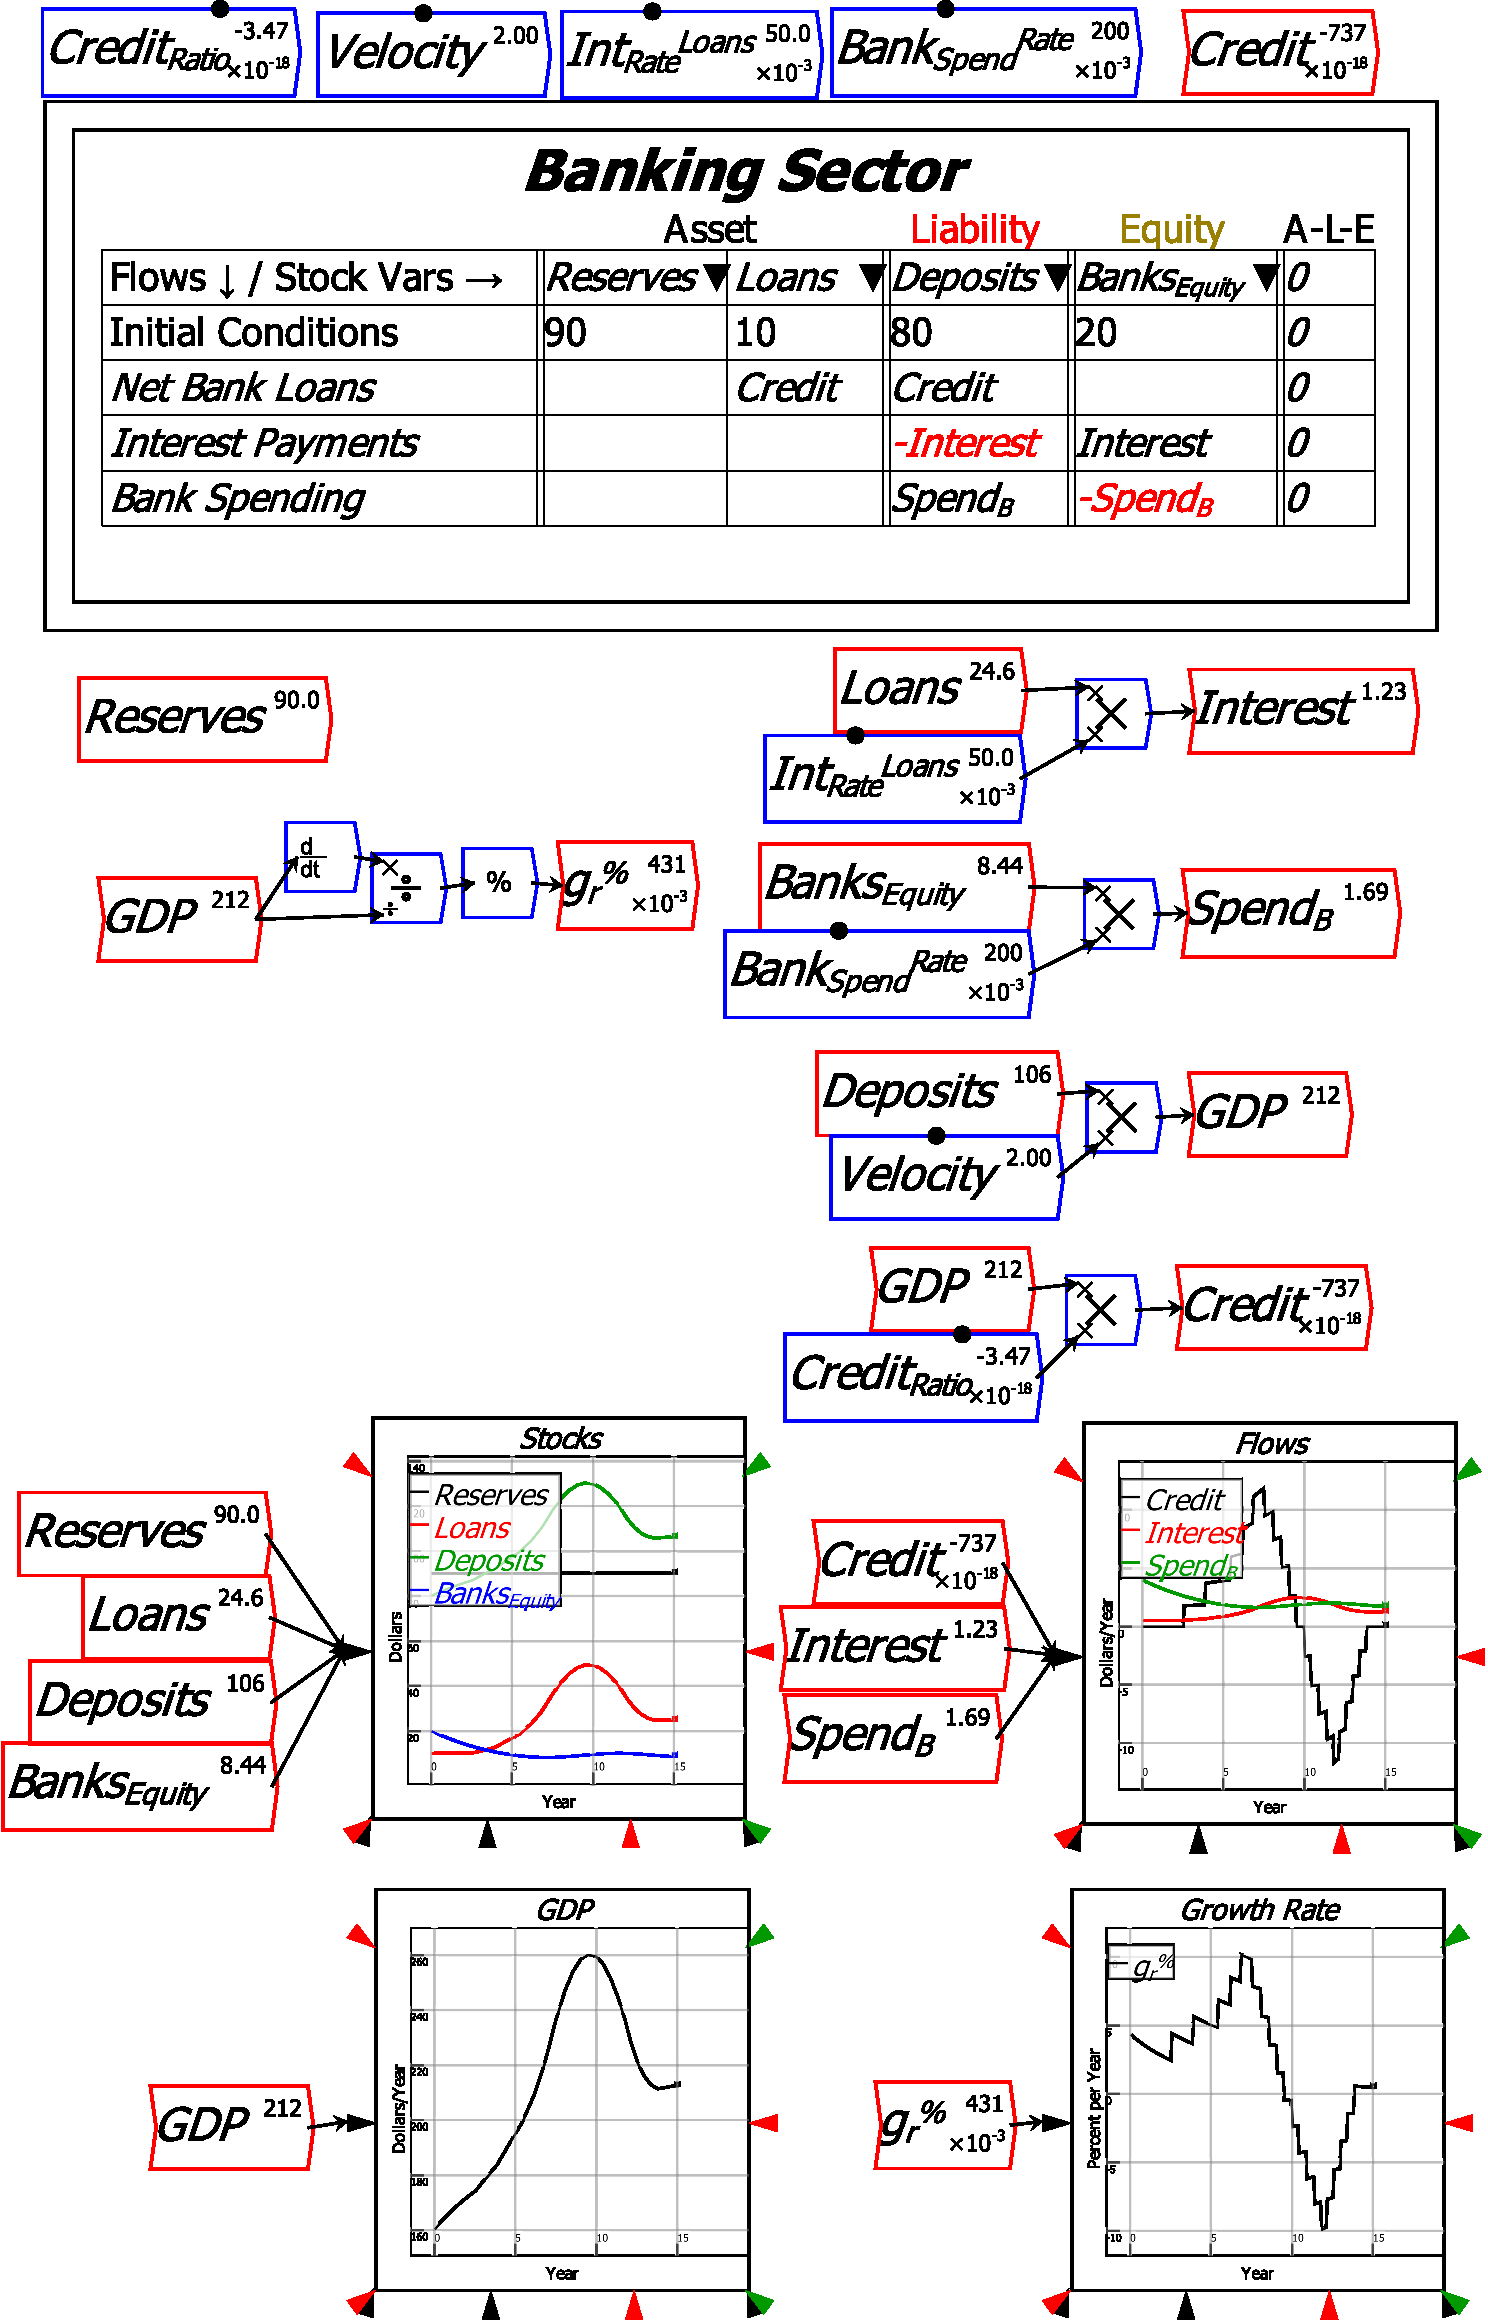
\includegraphics{images/MonetaryModel01GodleyTable07GDP}

Much more sophisticated models can be built using \emph{Minsky}, including
models that mix the flowchart method with Godley Tables to generate
models of both the physical and monetary systems.
